% --------------------------------------------------------------------
% Beamer Template 
% --------------------------------------------------------------------
% Necessary infos for documentstyle
\documentclass[compress]{beamer}

\usetheme{Stud}
\usepackage{times}
\usepackage[utf8]{inputenc}
\usepackage[T1]{fontenc} % nicht benoetigt, in folien wird eh nicht getrennt
\usepackage{ngerman}
\usepackage{graphicx}
%\usepackage{color}% color wird bereits von beamer geladen
\usepackage{verbatim}
\usepackage{psfrag}
\usepackage{math}
\usepackage{calc}
\usepackage{tabularx}
\usepackage{enumerate}


% --------------------------- Helpers ----------------------------
% to use these texts in two languages
% changes the parameter within {#}
% 1 = German
% 2 = English
\def\twolang#1#2{#1} 
\let\2=\twolang

% --------------------------------------------------------------------


\bibliographystyle{alphadin}
\graphicspath{{images/}}


% --------------------------------------------------------------------
\title{Reaktive Konstruktion eines planaren, euklidischen t-Spanners mit konstantem Ausgangsgrad}
\subtitle{Antrittsvortrag zur Bachelorarbeit}
\author[T. Budweg]{Tim Budweg}
\institute{
  \texttt{tbudweg@uni-koblenz.de} \\
  \vspace{0.2cm}
  \2{AG Rechnernetze\\
  Universität Koblenz-Landau}{Institute for Computer Science\\
  University of Koblenz and Landau}
}
\date{3. Juni 2015}
% --------------------------------------------------------------------



% document
\begin{document}

\frame{\titlepage}

%\logo{...} erst hier, damit es nicht mit auf die Titelseite kommt!
\logo{\pgfuseimage{logo}}

%\part{Overview}
%\section{\2{Überblick}{Overview}}
%\frame{
%  \frametitle{\2{Überblick}{Overview}}
%  \tableofcontents[part=2,hideallsubsections]
%}

% ====================================================================
% ====================================================================

% here comes the real content which is part of scontent.tex
\part{Content}

% ---------------------------------------------------------------------------
% - For showing graphics and text on one slide use:
%   \begin{columns}[T]
%	\begin{column}[T]{.5\linewidth}
%	    \includegraphics[width=\linewidth]{<filename>}
%	\end{column}
%	\begin{column}[T]{.5\linewidth}
%	    <content>
%	\end{column}
%   \end{columns}
% ---------------------------------------------------------------------------

\section{Einleitung}

\subsection{}
\begin{frame}
\frametitle{Verwandte Arbeiten}
\begin{itemize}
	\item reaktive Algorithmen, welche planare, zusammenhängende Graphen erzeugen (\emph{rPDT}, GDBF, BFP)
	%ohne t-Spanner->mögliche lange Umwege
	\item lokale Algorithmen mit konstantem Ausgangsgrad und euklidischer Spanner Eigenschaft (Modified Yao Step, \ldots)
\end{itemize}
\end{frame}

\subsection{}
\begin{frame}
\frametitle{Motivation}
\begin{itemize}  %energieeffizientes broadcast, recovery routing 
	\item energieeffiziente Konstruktion der Topologie
	\item für energieeffizientes Recovery-, Broadcastrouting, \ldots
\end{itemize}
\end{frame}
\subsection{}
\begin{frame}
\frametitle{Modified Yao Step}
	\begin{itemize}
		\item $LDel^{(2)}(U) $
		\item Modified Yao Step 
	\end{itemize}
\end{frame}

\subsection{}
\begin{frame}
\frametitle{$LDel^{(2)}(U) $}
\begin{itemize}
    \begin{columns}[T]
	\begin{column}[T]{.5\linewidth}
    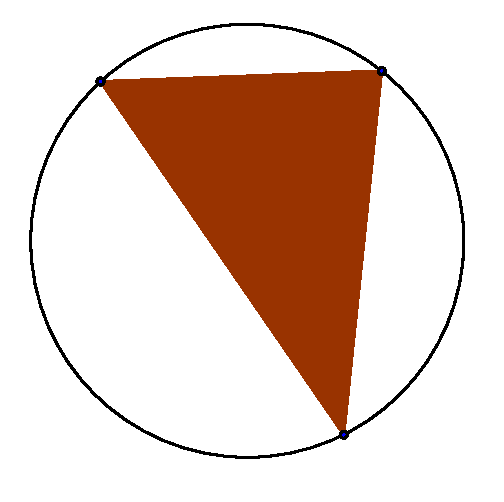
\includegraphics[width=\linewidth]{Dreieck.eps}
	\end{column}
	\begin{column}[T]{.5\linewidth}
	    \item alle Dreiecke, welche keine 2-Hop-Nachbarn in ihrem Umkreis beinhalten
	    \item vereinigt mit allen Kanten des Gabriel Graphen
	    
	\end{column}
   \end{columns}
\end{itemize}
\end{frame}

\subsection{Modified Yao Step}
\begin{frame}
  Input: $LDel^{(2)}(U) $
	\begin{itemize}
    \begin{columns}[T]
	\begin{column}[T]{.5\linewidth}
    \includegraphics[width=\linewidth]{finished_A.eps}
	\end{column}
	\begin{column}[T]{.5\linewidth}
	    \item Bilde Kegel
	    \item Wähle Kanten aus
	    \item Überprüfen der Kanten durch Kantenendpunkte
	    \item zusammenhängender, planarer, euklidischer t-Spanner mit konstantem Ausgangsgrad
	\end{column}
   \end{columns}
	\end{itemize}
\end{frame}

\section{Ziele}
\subsection{}
\begin{frame}
\frametitle{reactive Modified Yao Step}
Folgende Eigenschaften müssen erfüllt sein:
\begin{itemize}
  \item Ergebnisgraph ist ein euklidischer t-Spanner
  \item Ergebnisgraph ist planar
  \item Der Knotenausgangsgrad ist konstant beschränkt
  \item reaktive Konstruktion des Graphen
  \begin{itemize}
  	\item reaktiv: beaconloser Algorithmus, der lokal arbeitet
  \end{itemize}
  
\end{itemize}
\end{frame}



\section{Bisherige Ergebnisse}
\subsection{}
\begin{frame} 
\frametitle{Bisherige Ergebnisse}
	\begin{itemize}
    \begin{columns}[T]
	\begin{column}[T]{.3\linewidth}
    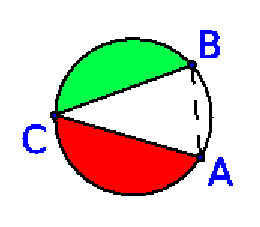
\includegraphics[width=\linewidth]{eigenschaft-beispiel.eps}
	\end{column}
	\begin{column}[T]{.7\linewidth}
	\item Beweis, dass PDT alle modified Yao Step Eigenschaften erfüllt, die $LDel^{(2)}(U) $ erfüllt
	\end{column}
   \end{columns}
	\end{itemize}
\end{frame}
% beispiel einfügen für eigenschaft

\subsection{}
\begin{frame}
\frametitle{reactive Modified Yao Step}
Input: planarer, t-spanner (PDT)\\
Output: zusätzlich konstanter Ausgangsgrad
	\begin{enumerate}
		\item bilde Kegel
		\item finde kürzeste Kante
		\item finde eine zusätzliche Kante für jeden leeren Kegel
		\item Prüfe, ob beide Endpunkte einer Kante diese akzeptieren
	\end{enumerate}
\end{frame}


\subsection{}
\begin{frame}
\frametitle{Existenz einer Kante bei beiden Endpunkte}
\begin{itemize}
	\item nicht sicher, ob nötig
	\item evtl. Ersetzung dieses Schrittes
\end{itemize}
\end{frame}

%hevorheben, dass der Beweis sehr wichtig ist!
\begin{frame}
\frametitle{Schritte}
\begin{itemize}
	\item beweisen, dass PDT geeignet ist $LDel^{(2)}(U) $ zu ersetzen
	\item entwerfen einer effizienteren Variante um die Existenz einer Kante bei beiden Eckpunkten zu überprüfen 
	\item Programmierung des Algorithmus in Sinalgo
\end{itemize}
\end{frame}

\begin{frame}
\frametitle{Zeitplan}
\begin{table}[h]
\resizebox{1.0\textwidth}{!}{%
\begin{tabular}{ll}
 Juni &   Beweis für PDT\\
 Juli &  Beweis für PDT, Programmierung\\
 August & Programmierung, effizientere Variante suchen \\
 September &Programmierung der neuen Variante, Vorbereiten des \\& Abschlussvortrags, Abgabe einer Vorabversion\\
 Oktober & Verbesserung und Abgabe der Finalversion,\\& Abschlussvortrag
\end{tabular}
}
\end{table}
\end{frame}
\end{document}